\chapter{Diskussion}

\subsection{Diskussion der Vorversuche}
Daraus l�sst sich schlie�en, dass Fisch 1 und Fisch 2 lernten, dass an den Elekrtroden Futter zu finden war.
Eine m�gliche Erkl�rung f�r den 'Zickzackkurs' von Fisch 3 und Fisch 4 w�re, dass sie nach einem erfolgreichen Versuchstag am n�chsten Tag keinen Hunger mehr hatten. Was dagegen spricht: F�tterung nur mit kleinen Larven und oftmals schlechte Leistungen an einem Montag, obwohl Fische gerade da hungrig sein sollten. Au�erdem waren das ja gerade die gro�en Fische, die sowieso mehr Futter brauchen sollten als die kleinen Fische.



\subsection{Diskussion der Relacsauswertung}

\subsubsection{S+ und s- vertauscht}

wenn man die stimuli bei 1mV und bei 2mV bei Fisch 2 'umdreht' ergibt sich:
overview: median: 50 Prozent, gewichtetes Mittel: 54,08 Prozent, P-Wert: 0,161
amplitude 1mV: median: 50, gewichtetes mittel: 54,08, p-wert: 0,2833
amplitude 2mV: median: 70, gewichtetes mittel: 66,67, p-wert: 0,029




\begin{table} [h] 
	\centering
	\caption{ Die Tabelle zeigt die S+ und S- Stimuli, auf welche die einzelnen Versuchstiere trainiert wurden. Das Fischsymbol (\PHtunny)  steht f�r ein eigenmanniaartiges Signal. Steht nichts hinter der angegebenen Beatfrequenz, handelt es sich um einen einfachen Stimulus.}
	\vspace{0,2cm}	
	\begin{tabular}{llll} %eigentliche Tabelle 
		\toprule % d�nne Linie 
		& S+ & S-\\
		 Fisch 1 (2015albi02):& +40 Hz & +40 Hz \PHtunny \\
		 Fisch 2 (2015albi01):& +60 Hz & +60 Hz \PHtunny \\
		 Fisch 3 (2014albi08):& - 60 Hz \PHtunny & - 60 Hz \\
		 Fisch 4 (2013albi14):& - 40 Hz \PHtunny & - 40 Hz \\
		 Fisch 5 (2013albi09):& +100 Hz & +100 Hz \PHtunny\\
		 Fisch 6 (2012albi01):& +40 Hz & +40 Hz \PHtunny \\
		\bottomrule % bi�chen dickere Linie unten
	\end{tabular}
	\label{beats}
\end{table}

warum k�nnte der S- stimulus f�r fisch 2 attraktiver sein? Nat�rliche Pr�ferenz?


\subsection{Diskussion der Trackingauswertung}

blablabla

Geschwindigkeitsboxplots: Fisch 4 und Fisch 6 generell schneller als Fisch 1 und 2. M�glicher Grund: Aufgeregt, unwohl gef�hlt auf offener Fl�che?

\begin{figure}[ht]
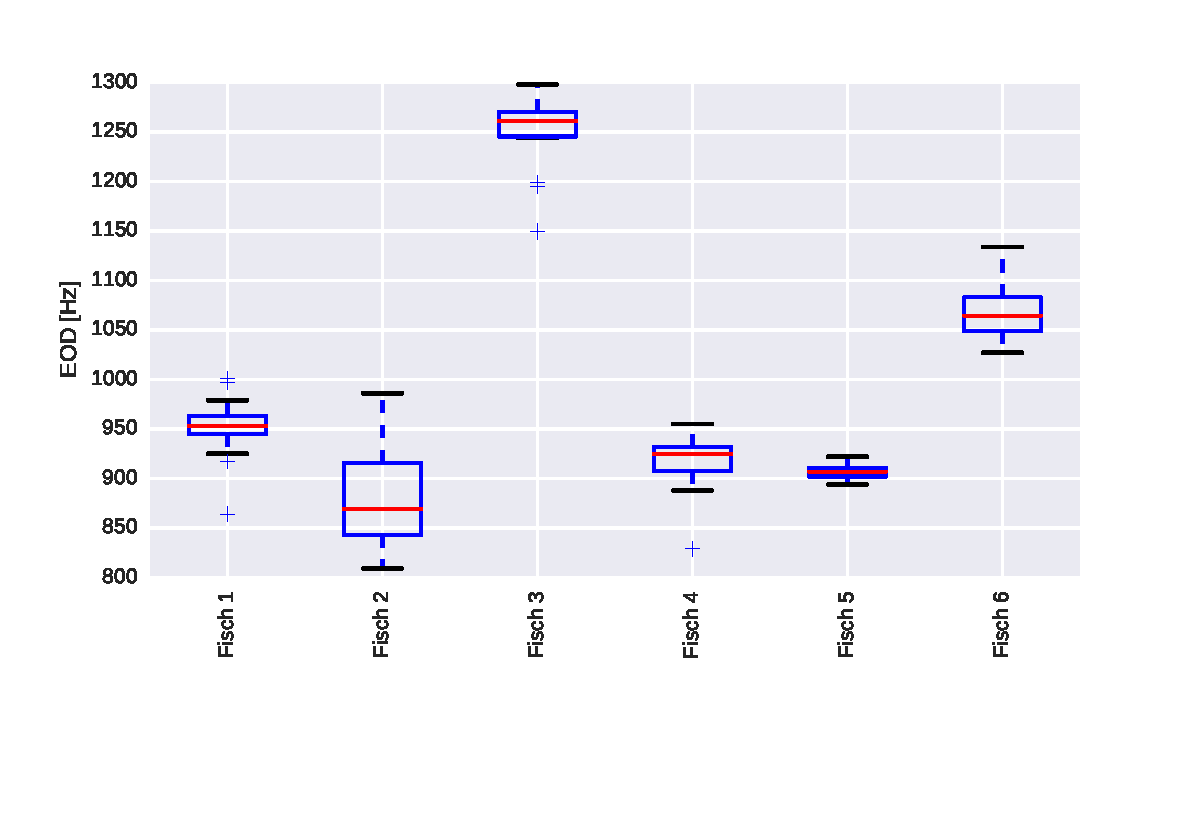
\includegraphics[height=8.5cm]{Abbildungen/eod_boxplot}
\caption{\label{fig:eods}Graphik zeigt die EOD Verteilung der Fische �ber den gesamten Versuchszeitraum inklusive Vorversuche.}
\end{figure}

Der EOD Median von Fisch 1 (siehe Abbildung \ref{fig:eods}) liegt dabei bei 953 Millivolt. Der Median von Fisch 2 hingegen liegt etwas tiefer und zwar bei 869 Millivolt. Fisch 3 hatte von allen Versuchstieren die h�chste EOD Frequenz und lag bei einem Median von 1261 Millivolt. Der Median von Fisch 4 befand sich bei 925 Millivolt und der von Fisch 5 bei 907 Millivolt. Fisch 6 besa� mit einem Median von 1064.5 Millivolt die zweit h�chste EOD Frequenz.


\begin{figure}[ht]
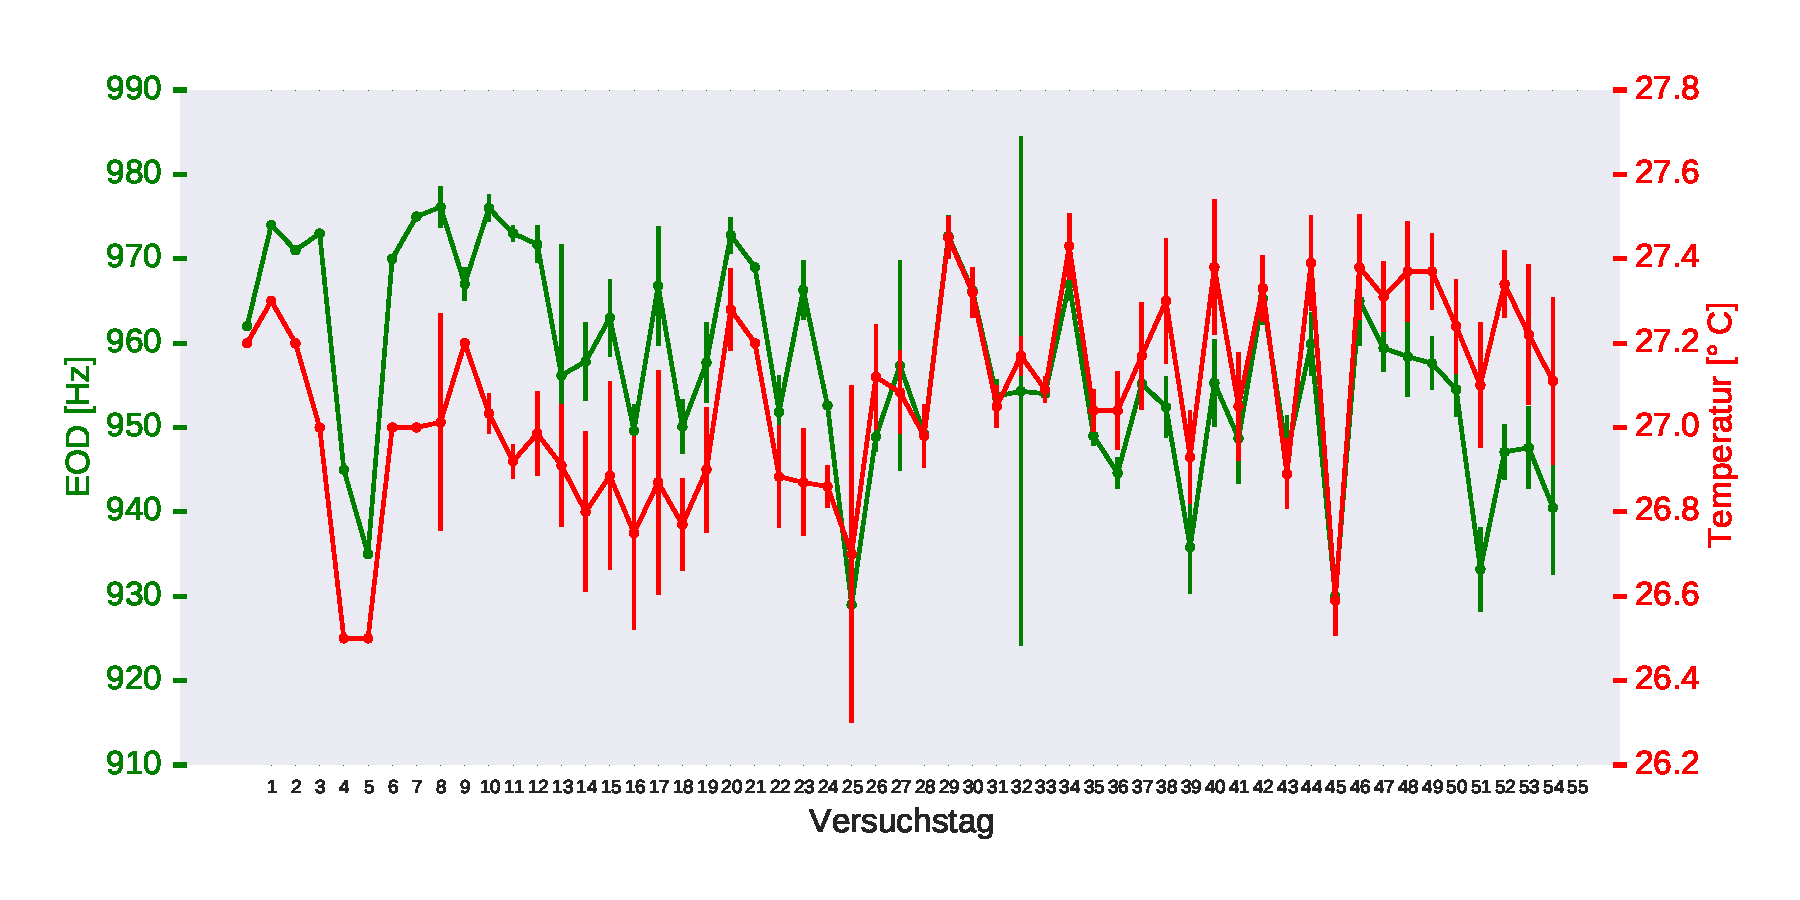
\includegraphics[height=6.5cm]{Abbildungen/date_temperature_eod_plot2015albi02}
\caption{\label{fig:temperatureod1}Die Graphik zeigt die Wassertemperaturen (rote Kurve) und die EOD Frequenzen von Fisch 1 in gr�n �ber die gesamte Versuchszeit einschlie�lich Vorversuche.}
\end{figure}

\begin{figure}[ht]
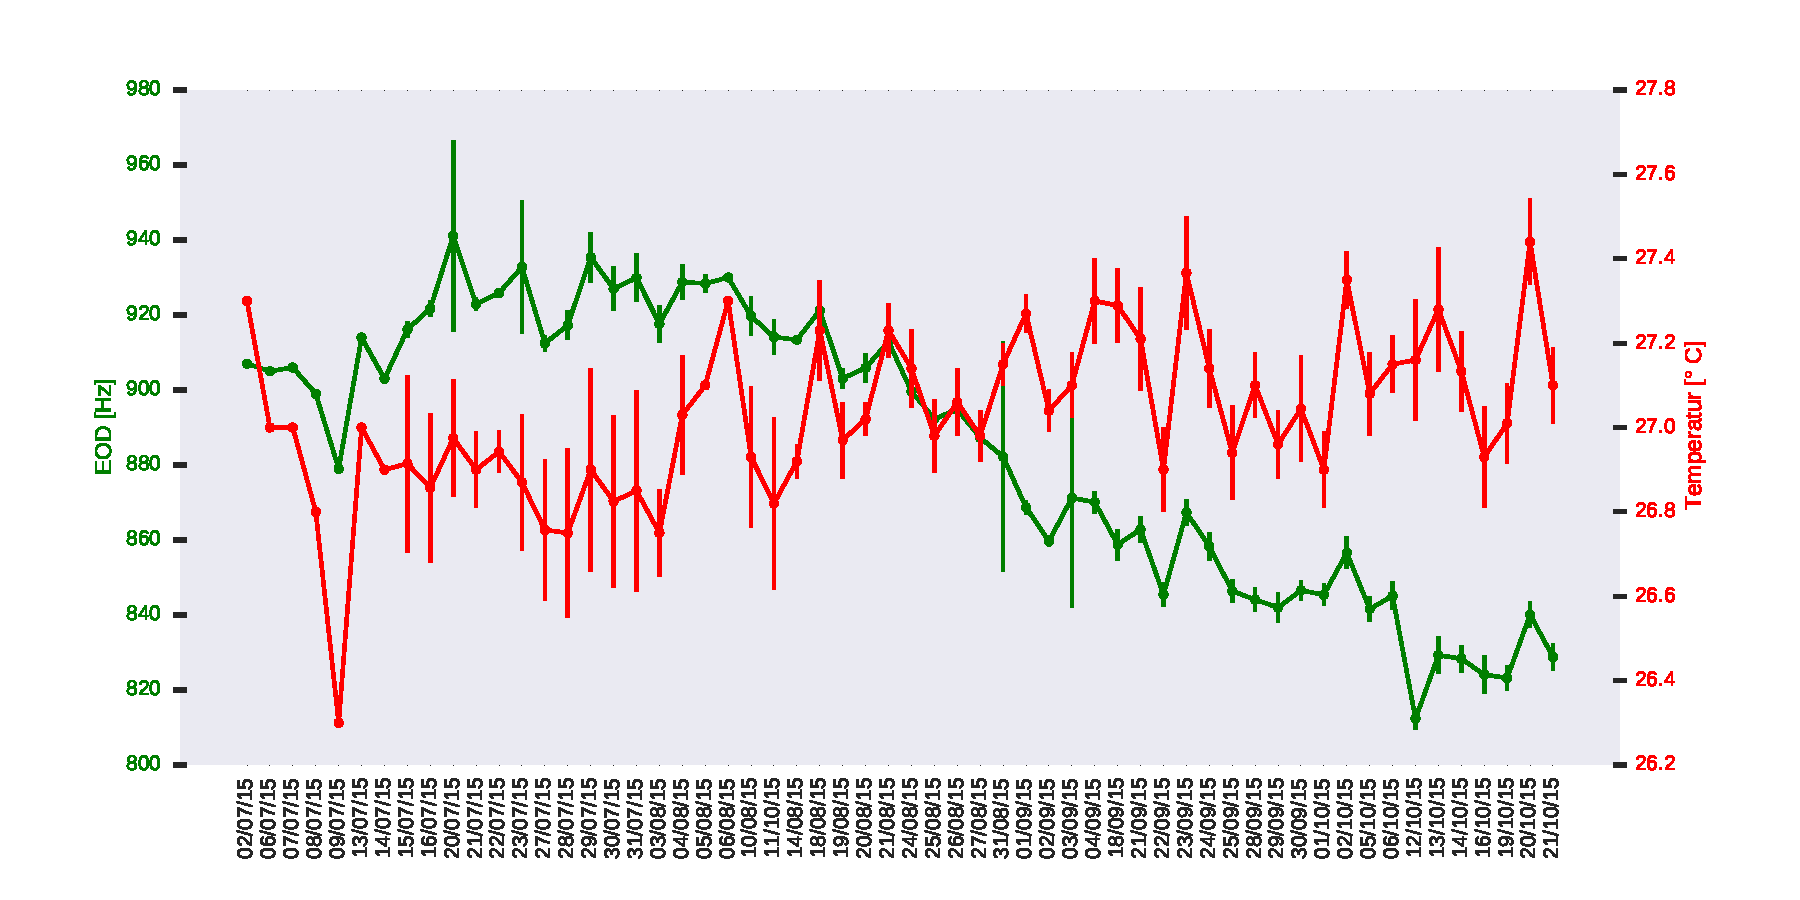
\includegraphics[height=6.5cm]{Abbildungen/date_temperature_eod_plot2015albi01}
\caption{\label{fig:temperatureod2}Die Graphik zeigt die Wassertemperaturen (rote Kurve) und die EOD Frequenzen von Fisch 2 in gr�n �ber die gesamte Versuchszeit einschlie�lich Vorversuche.}
\end{figure}


\begin{figure}[ht]
\subfigure[Fisch 3]
{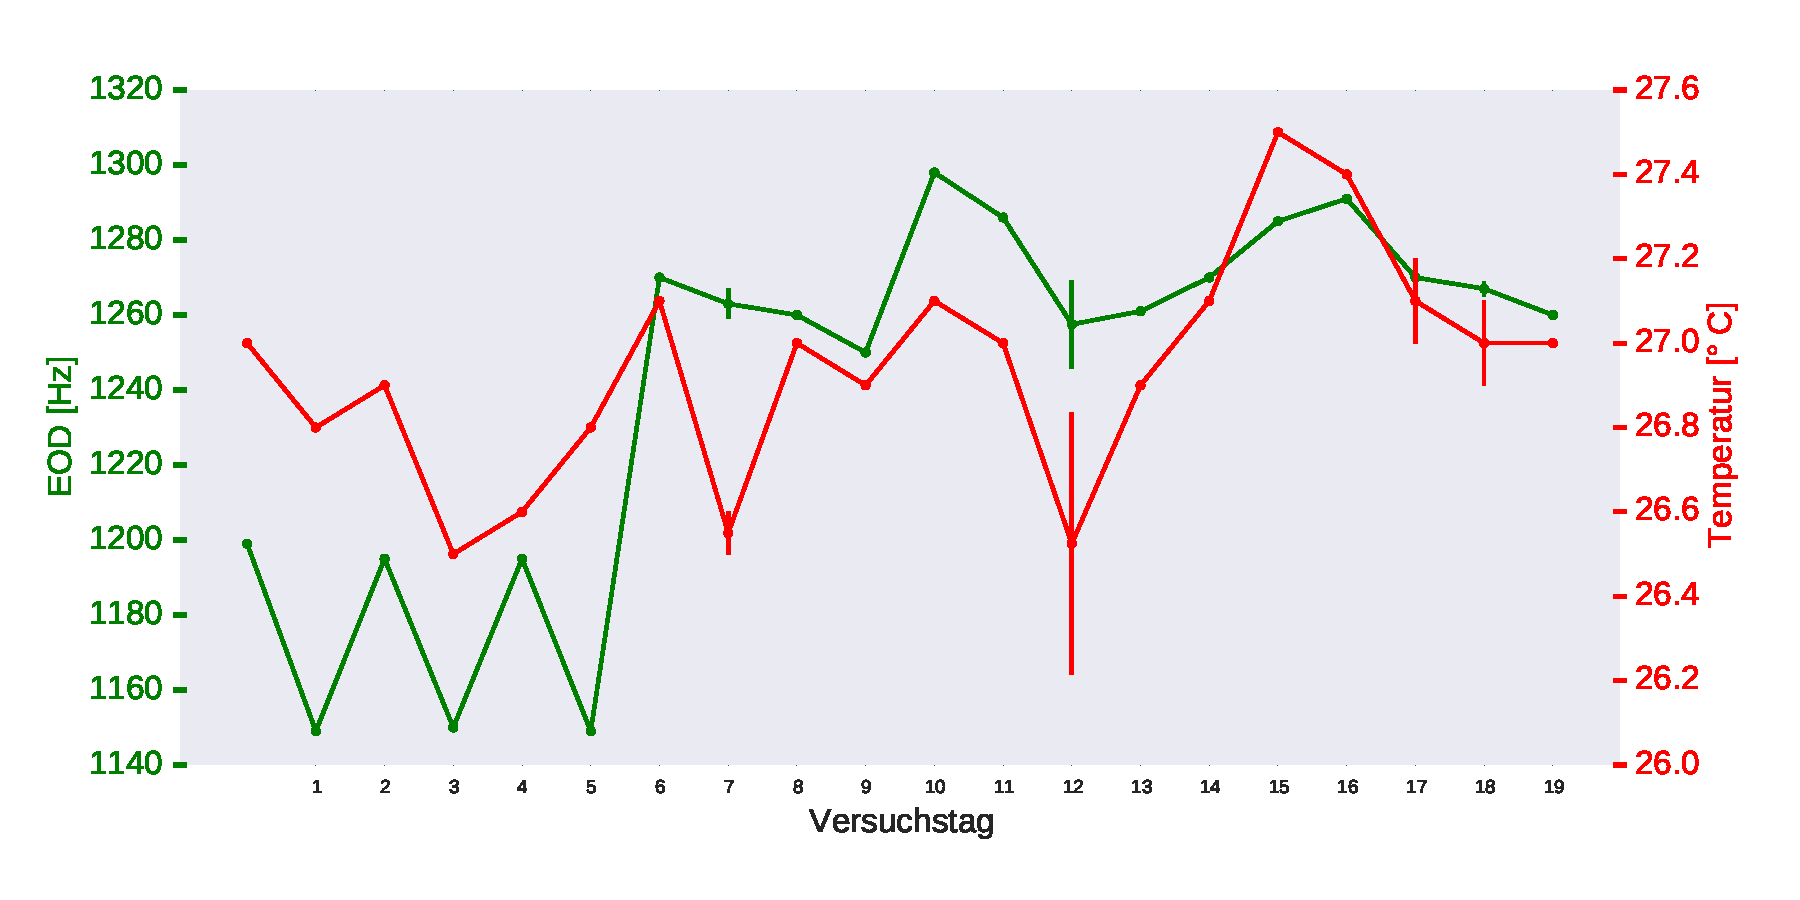
\includegraphics[height=4cm]{Abbildungen/date_temperature_eod_plot2014albi08}}
\subfigure[Fisch 4]
{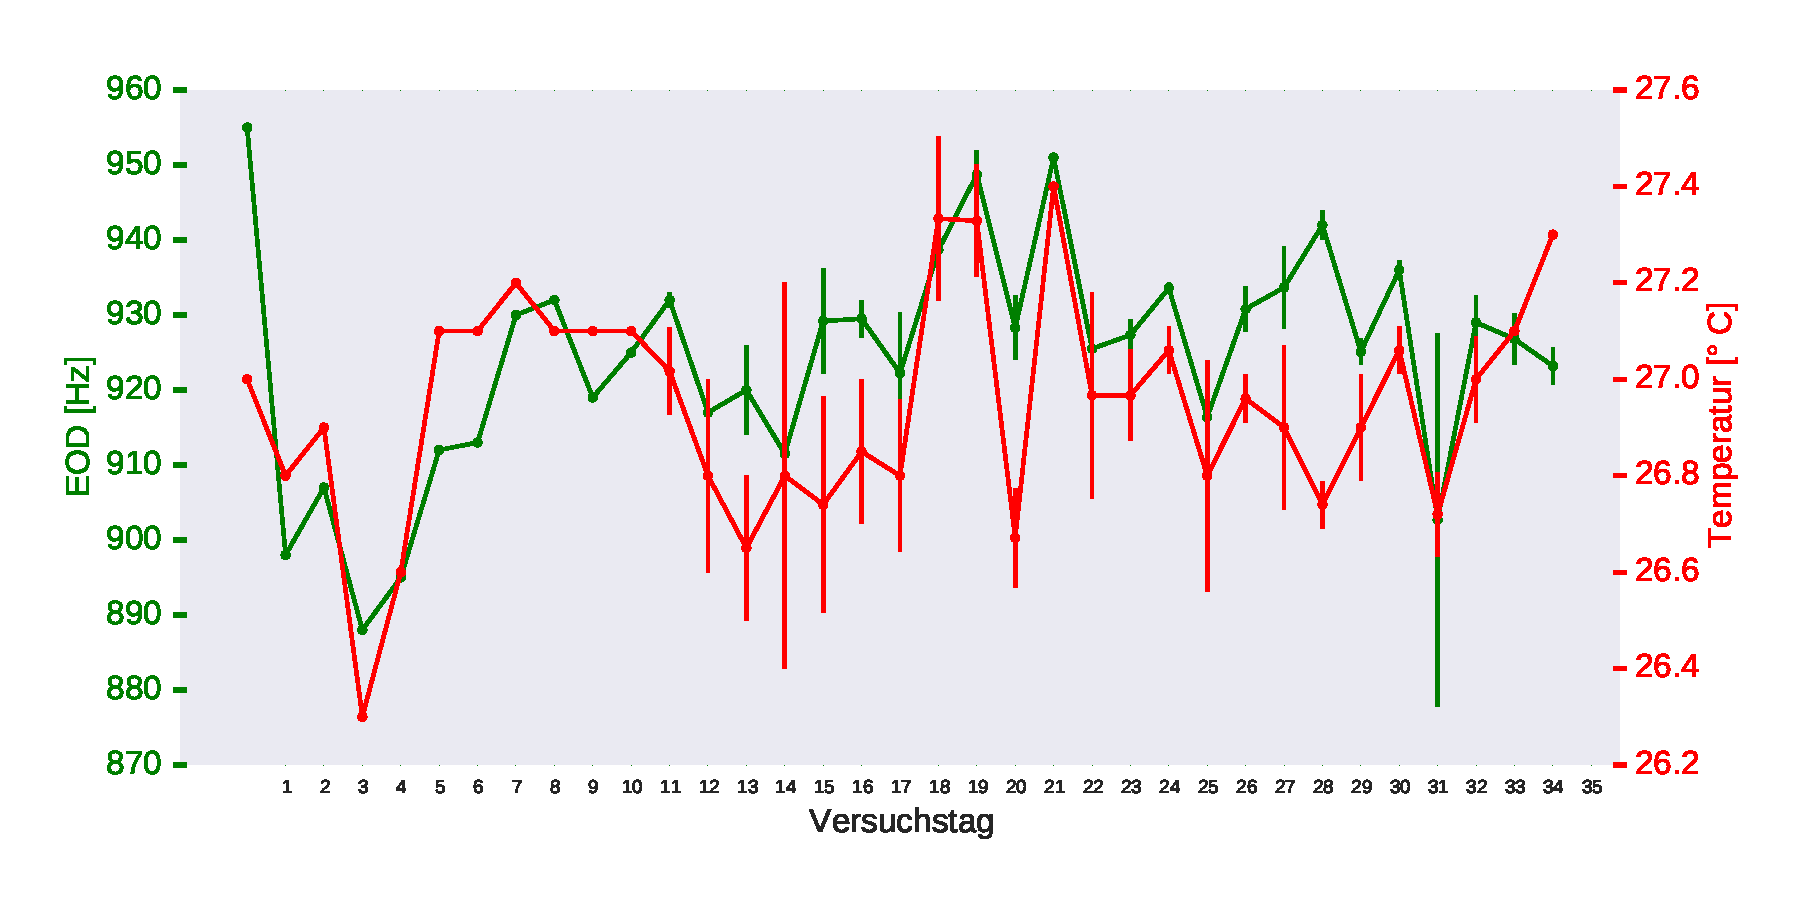
\includegraphics[height=4cm]{Abbildungen/date_temperature_eod_plot2013albi14}}
\subfigure[Fisch 5]
{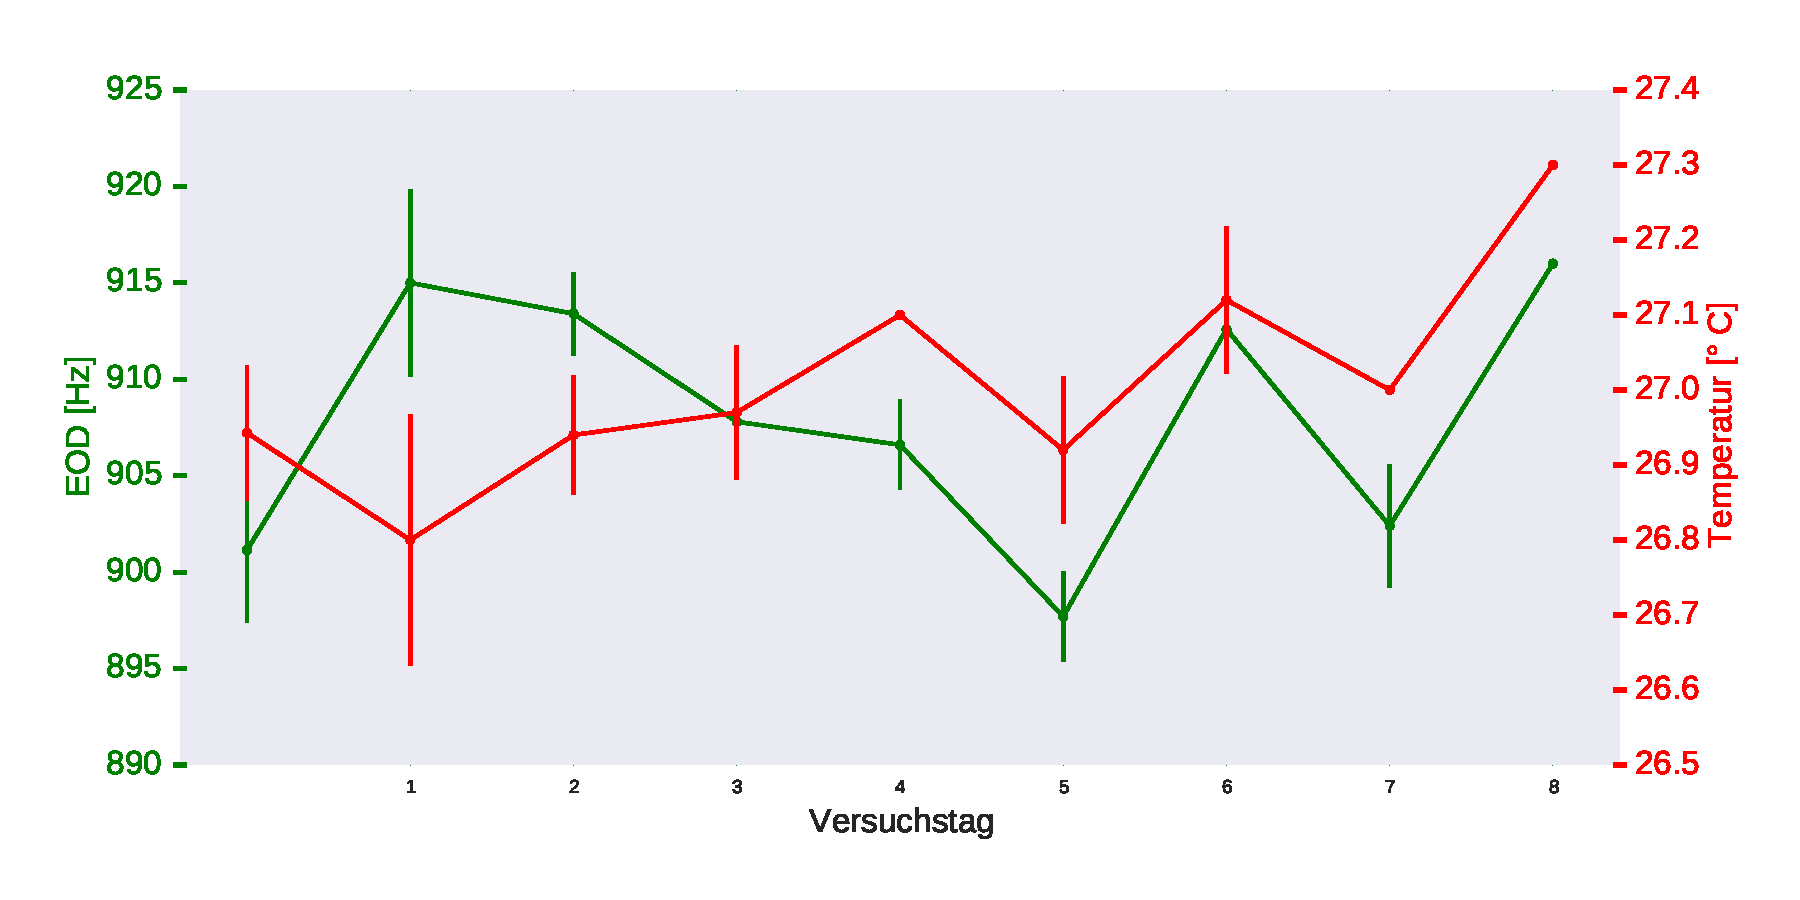
\includegraphics[height=4cm]{Abbildungen/date_temperature_eod_plot2013albi09}}
\subfigure[Fisch 6]
{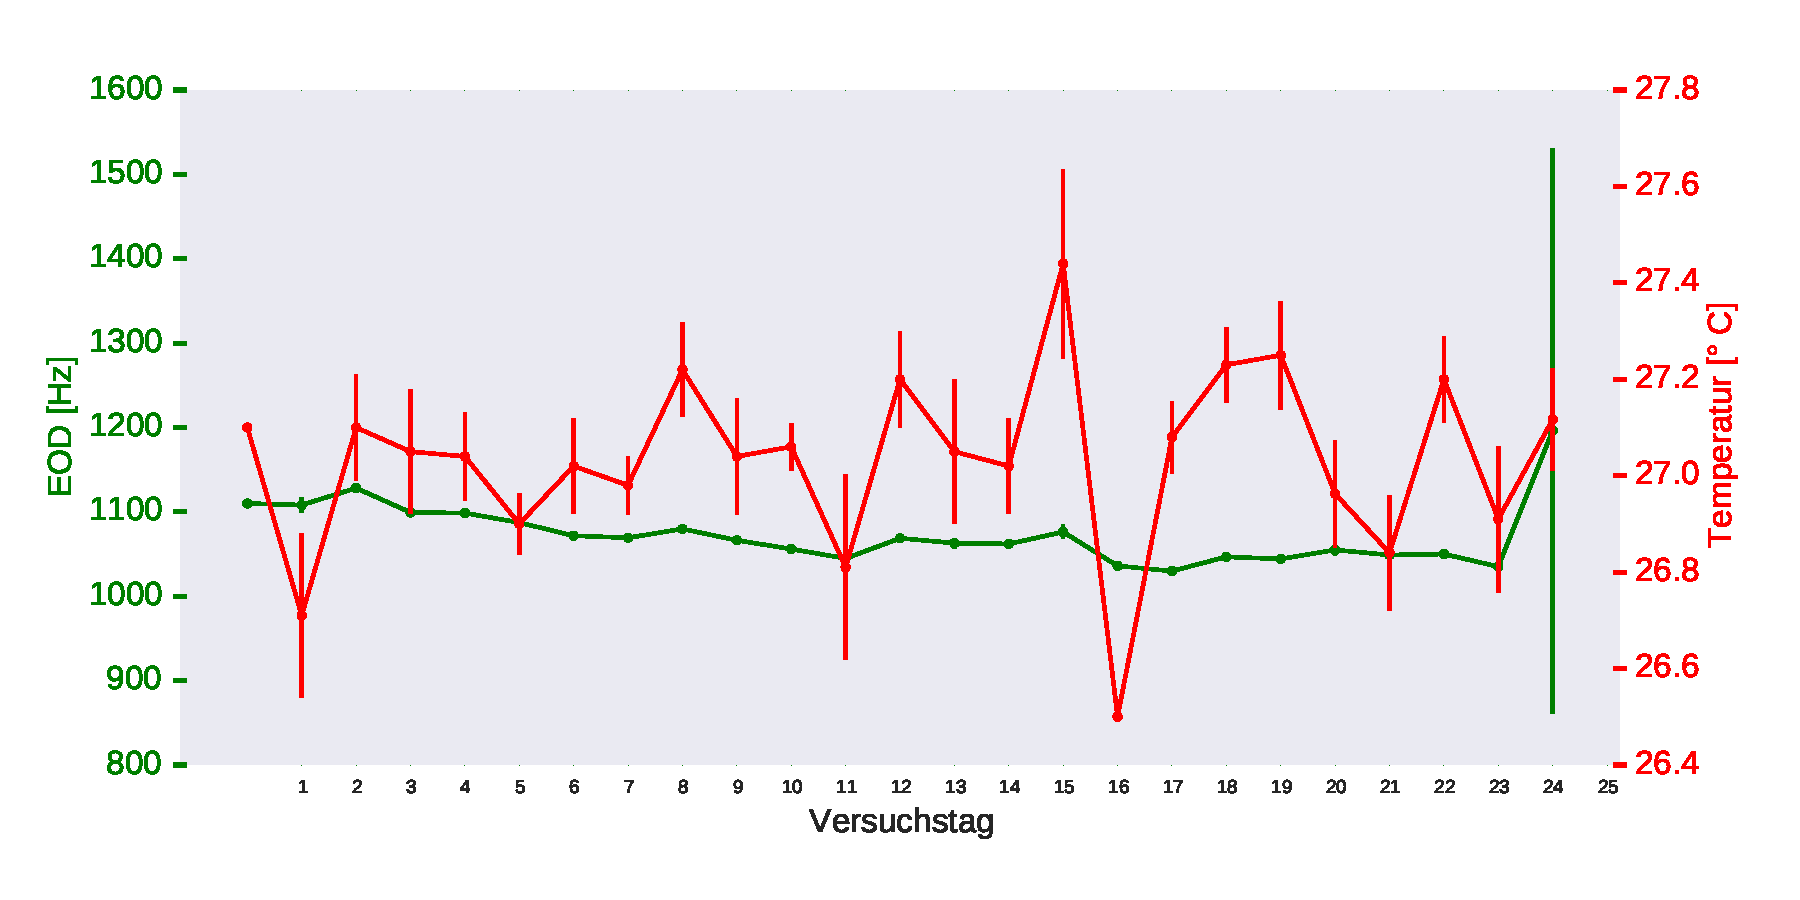
\includegraphics[height=4cm]{Abbildungen/date_temperature_eod_plot2012albi01}}
\caption{\label{fig: temperatureod3}  Wassertemperaturen (rote Kurve) und die EOD Frequenzen von Fisch 3, 4, 5, 6 in gr�n �ber die gesamte Versuchszeit einschlie�lich Vorversuche.}
\end{figure}


\begin{figure}[ht]
\subfigure[Fisch1]
{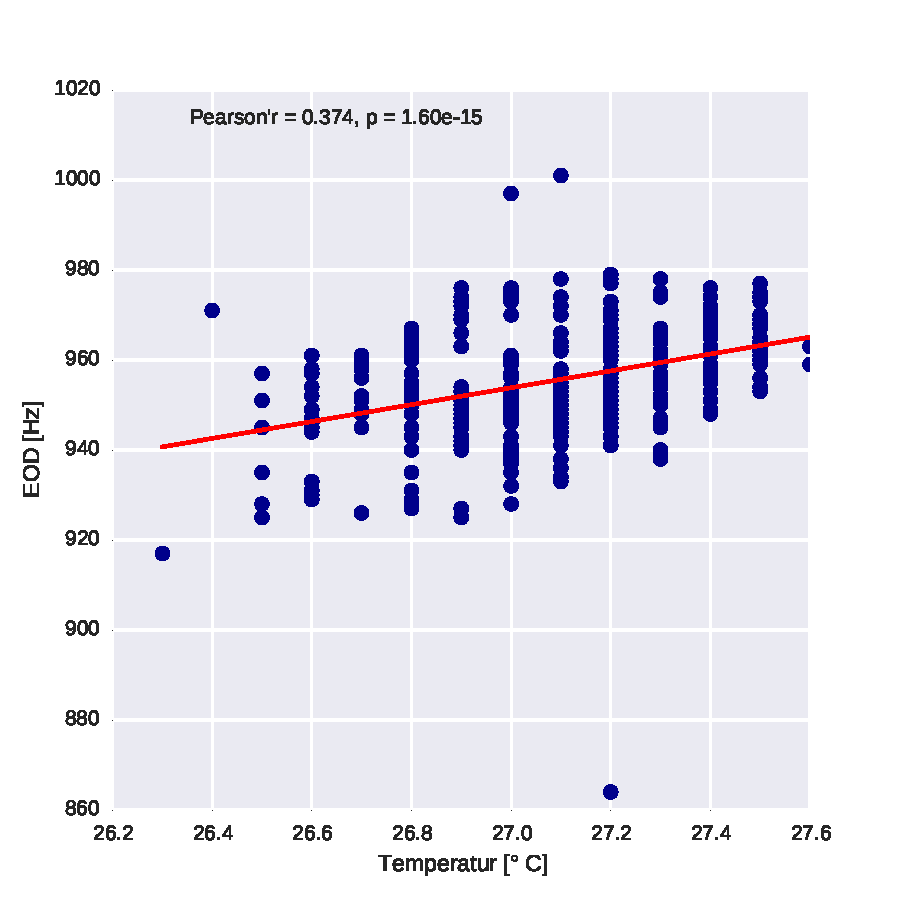
\includegraphics[height=6cm]{Abbildungen/regression1}}
\subfigure[Fisch2]
{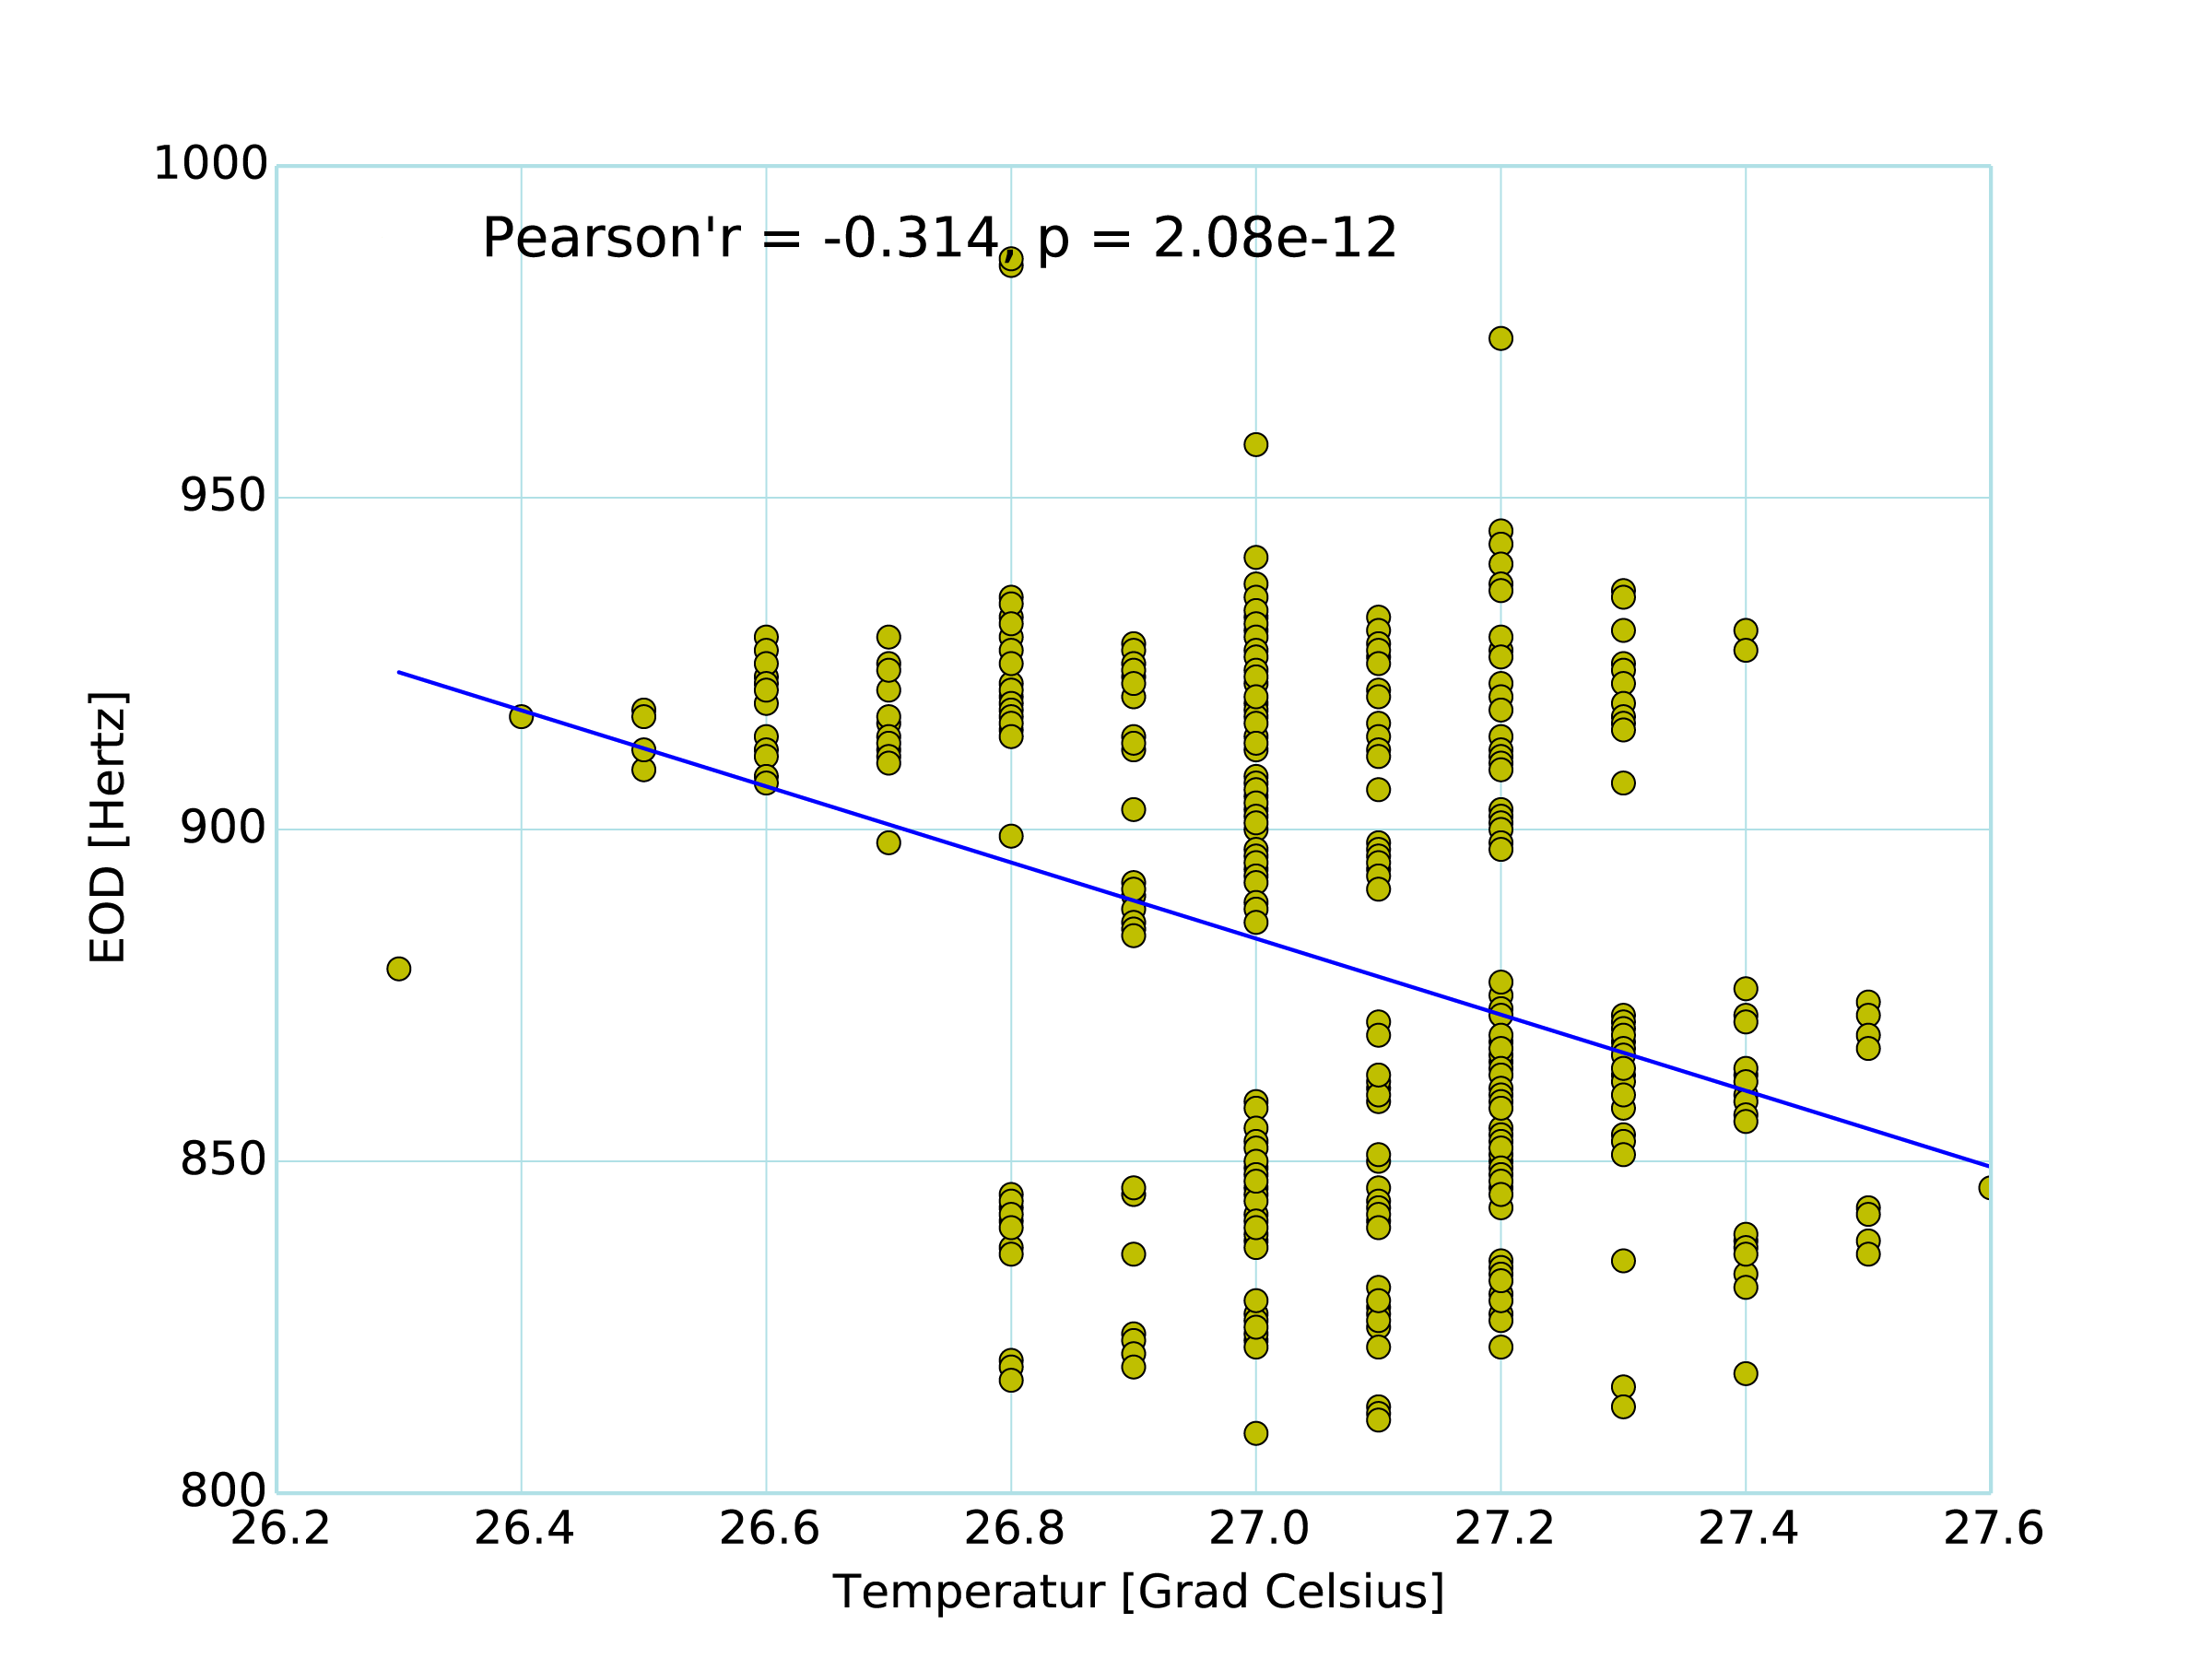
\includegraphics[height=6cm]{Abbildungen/regression2}}
\caption{\label{fig:regression}Regressionsgeraden von Temperatur und EOD.}
\end{figure}



\section{Vorversuche}
\subsection{Eingew�hnung}

Fish 1 und Fisch 2 gingen nach 9 Versuchstagen in die n�chste Phase die "Konditionierung auf den gew�nschten Reiz" �ber. Da Fisch 3 und Fisch 4 schlechter kooperierten, ginge diese erst nach elf Versuchstagen in die n�chste Phase �ber.


Paper Konditionierung?

